% generated by make_figs.mjs
\resizebox{\columnwidth}{!}{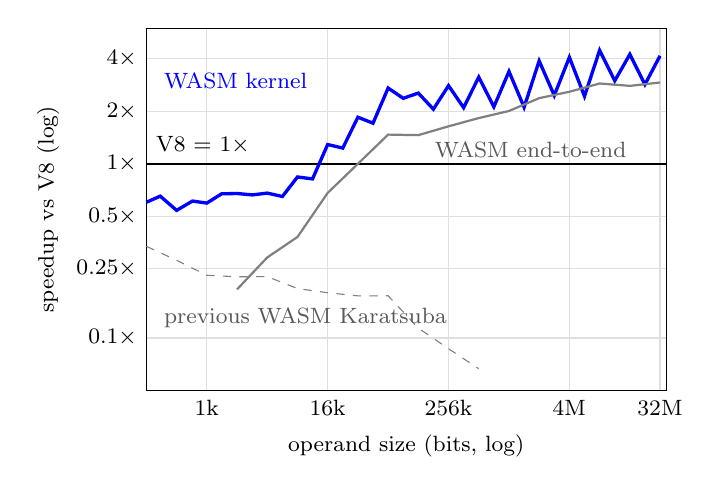
\begin{tikzpicture}[font=\footnotesize]
\draw[gray!25] (0,0.666) -- (6.6,0.666); \node[left] at (0,0.666) {$0.1\times$};
\draw[gray!25] (0,1.546) -- (6.6,1.546); \node[left] at (0,1.546) {$0.25\times$};
\draw[gray!25] (0,2.212) -- (6.6,2.212); \node[left] at (0,2.212) {$0.5\times$};
\draw[gray!25] (0,2.878) -- (6.6,2.878); \node[left] at (0,2.878) {$1\times$};
\draw[gray!25] (0,3.544) -- (6.6,3.544); \node[left] at (0,3.544) {$2\times$};
\draw[gray!25] (0,4.210) -- (6.6,4.210); \node[left] at (0,4.210) {$4\times$};
\draw[gray!25] (0.767,0) -- (0.767,4.6); \node[below] at (0.767,0) {1k};
\draw[gray!25] (2.302,0) -- (2.302,4.6); \node[below] at (2.302,0) {16k};
\draw[gray!25] (3.837,0) -- (3.837,4.6); \node[below] at (3.837,0) {256k};
\draw[gray!25] (5.372,0) -- (5.372,4.6); \node[below] at (5.372,0) {4M};
\draw[gray!25] (6.523,0) -- (6.523,4.6); \node[below] at (6.523,0) {32M};
\draw (0,0) rectangle (6.6,4.6);
\node at (3.3,-0.7) {operand size (bits, log)};
\node[rotate=90] at (-1.25,2.3) {speedup vs V8 (log)};
\draw[black,thick] (0,2.878) -- (6.6,2.878);
\node[anchor=south west] at (0.000,2.878) {V8 = $1\times$};
\draw[blue,very thick] plot coordinates {(0.000,2.390) (0.176,2.467) (0.384,2.287) (0.585,2.405) (0.767,2.379) (0.956,2.497) (1.151,2.501) (1.346,2.483) (1.535,2.506) (1.727,2.463) (1.919,2.711) (2.110,2.686) (2.302,3.123) (2.494,3.078) (2.686,3.470) (2.878,3.394) (3.070,3.840) (3.262,3.710) (3.453,3.776) (3.645,3.572) (3.837,3.871) (4.029,3.591) (4.221,3.979) (4.413,3.602) (4.605,4.051) (4.797,3.596) (4.988,4.185) (5.180,3.746) (5.372,4.231) (5.564,3.736) (5.756,4.320) (5.948,3.933) (6.140,4.269) (6.331,3.885) (6.523,4.249)};
\draw[gray,thick] plot coordinates {(1.151,1.283) (1.535,1.689) (1.919,1.949) (2.302,2.508) (2.686,2.878) (3.070,3.249) (3.453,3.242) (3.837,3.354) (4.221,3.459) (4.605,3.549) (4.988,3.712) (5.372,3.793) (5.756,3.898) (6.140,3.868) (6.523,3.911)};
\draw[gray,dashed] plot coordinates {(0.000,1.830) (0.384,1.653) (0.767,1.463) (1.151,1.443) (1.535,1.446) (1.919,1.293) (2.302,1.241) (2.686,1.201) (3.070,1.202) (3.453,0.792) (3.837,0.530) (4.221,0.276)};
\node[blue,anchor=west] at (0.101,3.934) {WASM kernel};
\node[gray!70!black,anchor=west] at (3.541,3.054) {WASM end-to-end};
\node[gray!70!black,anchor=west] at (0.101,0.918) {previous WASM Karatsuba};
\end{tikzpicture}}
